% Compile: pdflatex preprocessing_pipeline.tex  (in this directory)
% Output: preprocessing_pipeline.pdf -> copy/symlink to figures/
\documentclass[tikz,border=2pt]{standalone}
\usepackage[T1]{fontenc}
\usepackage{helvet}
\renewcommand{\familydefault}{\sfdefault}
\usepackage{tikz}
\usetikzlibrary{arrows.meta, positioning, shapes.geometric, fit}

\definecolor{accent}{HTML}{2E5A88}
\definecolor{accent2}{HTML}{1F6F54}
\definecolor{stepbg}{HTML}{EAF1F8}
\definecolor{stepbd}{HTML}{2E5A88}

\tikzset{
  stepbox/.style={
    draw=stepbd, fill=stepbg, rounded corners=3pt,
    minimum width=2.35cm, minimum height=0.95cm,
    align=center, font=\footnotesize, inner sep=4pt
  },
  arr/.style={-{Stealth[length=2.2mm]}, thick, color=accent!80}
}

\begin{document}
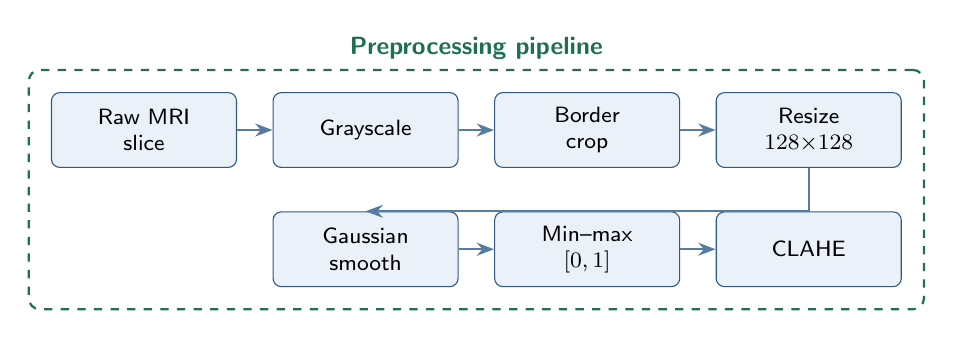
\begin{tikzpicture}[node distance=0.55cm and 0.45cm]
  \node[stepbox] (raw) {Raw MRI\\slice};
  \node[stepbox, right=of raw] (gray) {Grayscale};
  \node[stepbox, right=of gray] (crop) {Border\\crop};
  \node[stepbox, right=of crop] (resize) {Resize\\$128{\times}128$};

  \node[stepbox, below=of gray] (smooth) {Gaussian\\smooth};
  \node[stepbox, right=of smooth] (norm) {Min--max\\$[0,1]$};
  \node[stepbox, right=of norm] (clahe) {CLAHE};

  \draw[arr] (raw) -- (gray);
  \draw[arr] (gray) -- (crop);
  \draw[arr] (crop) -- (resize);
  \draw[arr] (resize.south) |- (smooth.north);
  \draw[arr] (smooth) -- (norm);
  \draw[arr] (norm) -- (clahe);

  \node[draw=accent2, thick, dashed, rounded corners=4pt,
        fit=(raw)(clahe), inner sep=8pt, label={[accent2, font=\small\bfseries]above:Preprocessing pipeline}] {};
\end{tikzpicture}
\end{document}
